\documentclass[11pt,a4paper,oneside]{memoir}

% Packages
\usepackage{geometry}
\usepackage{graphicx}
\usepackage{enumerate}
\usepackage{amsmath}
\usepackage{amssymb}
\usepackage{amsfonts}
\usepackage{amsthm}
\usepackage{float}
\usepackage[T1]{fontenc}
\usepackage[
    colorlinks=true,
    %linkcolor=blue, urlcolor=blue, citecolor=blue % pdf
    linkcolor=black, urlcolor=black, citecolor=black % print
]{hyperref}

% Set correct spacing between lines
\OnehalfSpacing
% Look for images under the .images/ dir
\graphicspath{ {./images/} }
% Specifiy stype for bibliography
\bibliographystyle{abbrv}

% Theorem and Proposition styling
\theoremstyle{plain}
% Reset theorem numbering for each chapter
\newtheorem{thm}{Theorem}[chapter]
% Reset definition numbering for each chapter
\newtheorem{prop}[thm]{Proposition}
% Reset definition numbering for each chapter
\newtheorem{lem}[thm]{Lemma}

% Definition and Example styling
\theoremstyle{definition}
% Definition numbers are dependent on theorem numbers
\newtheorem{defn}[thm]{Definition}
% Example numbers are dependent on theorem numbers
\newtheorem{exmp}[thm]{Example}

\begin{document}

% -------------- TITLE PAGE --------------
\begin{titlingpage}
    \centering
        \vspace*{3cm}
 
        \Huge
        \textbf{Chaos in Discrete Dynamical Systems}
             
        \vspace{1.5cm}
        
        \LARGE
        \textit{Fraser Love}
             
        \vspace{1.5cm}
             
        \Large
        School of Mathematics and Statistics\\
        University of St Andrews\\

        \vfill

        {\large \today\par}
 \end{titlingpage}
% ------------ TITLE PAGE END ------------

\noindent\textit{I certify that this project report has been written by me, is a record of work carried out by me, and is essentially different from work undertaken for any other purpose or assessment.}

\vspace{0cm}\hspace{12.8cm}
\includegraphics[width=1.3cm]{signature}

\begin{abstract}
    \noindent What is Chaos? How does it arise? This project explores chaotic discrete dynamical systems through the lense of pure Mathematics. We will start by defining discrete dynamical systems and give examples to show how chaos can arise in the simplest of systems. We will then go on to define the many notions of chaos in a dynamical system and explore numerous examples of chaotic discrete systems. Moreover we will explore the beautiful chaos of chaotic attractors and fractals. The mathematics in this paper is aimed at an interested undergraduate student with a solid understanding of calculus and real analysis.
\end{abstract}

\tableofcontents

\chapter{One-Dimensional Dynamics}

\section{Discrete Dynamical Systems} \label{sec:dynsys}

Discrete dynamical systems are eveywhere in Mathematics. A discrete dynamical system is defined as a set and a continuous function from this set to itself whereby points in this set are \emph{mapped} to other points in the same set by the application of this function. We will find out later how such systems can exhibit dynamical, complex irregular that we shall define as \emph{chaotic} and explore how this behaviour arises. Initially we will be working with discrete systems that are defined by one-dimensional functions, also called \emph{maps} or \emph{mappings}. However, in later chapters we shall explore higher dimensional dynamical systems. We shall start with defining what a discrete dynamical system is and look at some basic examples.

\begin{defn}
    Let $I$ be a non-empty compact set. A \emph{discrete dynamical system} is given by a continous map $f: I \to I$. The system starts at a point $x$ and evolves through iterative applications of the map $f$ on points in $I$. After $n$ iterations of $f$ the system can be described by $f^n := f \circ f \circ \cdots \circ f$ where $n \in \mathbb{N}$. By convention we take $f^0$ to be the identity map. Any point $x_n \in I$ in the system can be described by the application of $f$ on its previous points as follows: $x_n = f(x_{n-1})$.
\end{defn}

\begin{exmp}
    One of the simplest discrete dynamical systems is the map: $f: \mathbb{R} \to \mathbb{R}$ where $f(x) = 2x$. Each new point can be calculated from the previous point by the equation $x_n = 2x_{n-1}$. Let $x_0$ be the initial value of the system. The value of the system after $n$ sucessive iterations of the map $f$ is given by $f^n(x_0) = 2^nx_0$. It is clear that this system grows exponentially and is unbounded.
\end{exmp}

\begin{exmp}
    A more interesting discrete system is the logistic map $f: [0,1] \to [0,1]$ where $f(x)=\mu x(1-x)$. Lets initially set $\mu = 2$ and hence $f(x) = 2x(1-x)$. For $x \ll 1$, $f(x) \simeq 2x$, however for $x \gg 0$, $f(x) \simeq 2(1-x) < 1$. It will be shown in Section \ref{sec:logistic_maps} that any initial $x_0 \in (0, 1)$ will be attracted towards the fixed point of $x = 1/2$. Surprisingly as the value of $\mu$ approaches a value of $4$ the logistic map displays complex, irregular behaviour which we will later define as chaotic. In Section \ref{sec:logistic_maps} we shall explore how this behaviour arises.
\end{exmp}

\section{Orbits and Periodicity}
Here we will introduce some elementary definitions that are central to our exploration into chaos in discrete dynamical systems. We will then apply these definitions to the simplest of discrete systems we have just introduced. The following definitions are adapted from Ruette, Section 1.2 \cite{ruette}.

\begin{defn}
    Let $f: I \to I$ be a map. The \emph{orbit} or \emph{forward orbit} of $x$ under $f$ is the set $\mathcal{O}_f(x) = \mathcal{O}^+_f(x) = \lbrace f^n(x) : n \geq 0 \rbrace = \lbrace x, f(x), f^2(x), \cdots \rbrace$ of iterates of $x$ under $f$. If the map $f$ is invertible with $f^{-1}$ continuous then the \emph{backward orbit} of $x$ under $f$ is similarly defined as $\mathcal{O}^-_f(x) = \lbrace f^n(x) : n \leq 0 \rbrace = \lbrace x, f^{-1}(x), f^{-2}(x), \cdots \rbrace$.
\end{defn}

\begin{defn}
    Let $f: I \to I$ be a map. The \emph{trajectory} of $x$ is the infinite sequence $(f^n(x))_{n \geq 0}$. If $x$ is \emph{periodic} there will be repetitions in this sequence.
\end{defn}

\begin{exmp}
    Let $f: \mathbb{R} \to \mathbb{R}$ where $f(x) = 2x$. Any $x \in \mathbb{R}$ has the trajectory $(2^nx)_n$ and orbit $\mathcal{O}_f(x) = \lbrace 2^nx \rbrace$ where $n \geq 0$.
\end{exmp}

\begin{defn}
    Let $f: I \to I$ be a map. A point $x \in I$ is \emph{fixed} if $f(x) = x$. Hence, for a fixed point the orbit $\mathcal{O}_f(x) = \lbrace x \rbrace$.
\end{defn}

\begin{defn}
    Let $f: I \to I$ be a map. A point $x \in I$ is \emph{periodic} if $f^n(x) = x$ for some $n \in \mathbb{N}$. The \emph{period} of a point $x$ is the least positive integer $p$ such that $f^p(x) = x$. If $x$ has a period of $p$ we say that $x$ is a period-$p$ point. Moreover, $f^n(x) = x \iff n = kp$ for some $k \in \mathbb{N}$ (i.e. $n$ is a multiple of $p$). Hence $\mathcal{O}_f(x) = \lbrace x, f(x), \cdots, f^{p-1}(x) \rbrace$ is a finite set of unique points.

\end{defn}

A fixed point is simply a point with period one. Hence, throughout this paper results that hold for periodic points will also hold for fixed points. The period-$k$ points in a system $f: I \to I$ can be found by solving $f^k(x) - x = 0$, where $x \in I$. Hence we can find fixed and periodic points in the following discrete systems.

\begin{exmp}
    For the identiy map $id: \mathbb{R} \to \mathbb{R}$ where $id(x) = x$, for all $x \in \mathbb{R}$. Hence every point $x \in \mathbb{R}$ is a fixed point.
\end{exmp}

\begin{exmp}
    The map $f: \mathbb{R} \to \mathbb{R}$ where $f(x) = -x$ has no fixed points as $f(x) \neq x$, $\forall x \in \mathbb{R}$. However, $f^2(x) = f(-x) = x$ so every point $x \in \mathbb{R} \backslash \lbrace 0 \rbrace$ is a period-$2$ point.
\end{exmp}

\begin{exmp}
The map $f: \mathbb{R} \to \mathbb{R}$ where $f(x) = 2x^2 - 3x$ has fixed points when $f(x) = 2x^2 - 3x = x \implies x = 0$ or $x = 2$. The maps period-2 points can be found by finding the solutions to $f^2(x) = 2(2x^2 -3x)^2 - 3(2x^2 - 3x) = x$. Hence $x = (1 - \sqrt{3}) / 2$ and $x = (1 + \sqrt{3})/2$ are period-2 points.
\end{exmp}

These next two definitions will allow us to define the behaviour of a larger class of discrete dynamical systems. Most discrete dynamical systems infact do not have simple periodic orbits but instead either enter a periodic orbit after a certain number of iterations of the map $f$ or converge asymptotically to a periodic orbit.

\begin{defn}
    Let $f: I \to I$ be a map. A point $x \in I$ is \emph{eventually periodic} of period $n$ if there exists a $m > 0$ such that $f^{n+k}(x) = f^k(x)$, $\forall k \geq K$.
\end{defn}

\begin{exmp}
    Let $f: \mathbb{R} \to \mathbb{R}$, $f(x) = x^2 - 1$. The point $\sqrt{2}$ is eventually periodic as $f^2(\sqrt{2}) = f(1) = 0$ and $0$ is a period-2 point as $f^2(0) = f(-1) = 0$.
\end{exmp}

\begin{prop}
    Let $f: I \to I$ be a map. If $f$ is invertible then every eventually periodic point is periodic.
    \begin{proof}
        Suppose $x \in I$ is eventually periodic in $f$. Then $f^{n+k}(x) = f^k(x)$ for some $k > 0$. By applying $f^{-1}$ a total of $K$ times we get $f^n(x) = x$. Hence $x$ is periodic with period $n$.
    \end{proof}
\end{prop}

\begin{defn}
    Let $f: I \to I$ be a map. A point $x \in I$ is \emph{forward asymptotic} of period $n$ if $\lim_{i \to \infty} f^{in}(x) = p$.
\end{defn}

\begin{exmp}
    Let $f: \mathbb{R} \to \mathbb{R}$, $f(x) = x^3$. Any point $x \in (-1, 1)$ is forward asymptotic of period one to the fixed point $x = 0$ as \[\lim_{i \to \infty} f^{i} \left(x\right)  = \lim_{i \to \infty} \left(x\right) ^{3i} = 0.\]
\end{exmp}

\section{Stability of Periodic Points}
The stability of periodic points is integral to the emergence of chaos in a discrete dynamical system. Periodic points that are stable attract nearby points and the system settles into a steady state. Unstable periodic points however cause nearby points to diverge and small pertubations can cascade into large differences. Here, we will define what it means for periodic points to be stable or unstable. The following results are adapted from Devaney, Section 1.4 \cite{devaney}.

\begin{defn}
    Let $x \in I$ be a periodic point with period $k$. The point $x$ is said to be \emph{hyperbolic} if $|(f^k)'(x)| \neq 1$.
\end{defn}

Now using this notion of a hyperbolic point we will define what it means for a periodic point $p$ to be attracting.

\begin{prop} \label{prop:attractor}
    Let $f: I \to I$ be smooth and $p \in I$ be a hyperbolic periodic point of period $k$ with $|(f^k)'(p)| < 1$. Then there exists an open interval $U$ with $p \in U$ such that if $x \in U$, then \[ \lim_{n \to \infty} f^n(x) = p \]

    \begin{proof}
        Let $p$ be a period-$k$ point. By the Mean Value Theorem, for all $x \in I$, there exists a $c \in I$ such that \[f^k(x) - f^k(p) = f^k(x) - p = (f^k)'(c)(x-p)\] Since $f'$ is continuous at $c$, there exists $\varepsilon > 0$ such that $|(f^k)'(c)| < A < 1$ for $c \in U = [p - \varepsilon, p + \varepsilon]$ and some $A \in \mathbb{R}$. Hence for some $x \in U$ \[|f^k(x) - p| = |f^k(x) - f^k(p)| \leq A|x-p| < |x-p| \leq \varepsilon\] Thus $f^k(x) \in U = [p - \varepsilon, p + \varepsilon]$. Moreover, since $|f^k(x) - p| < |x - p|$, $f^k(x)$ is closer to $p$ than $x$ is. Applying this same argument inductively we deduce that if $n = mk$ for some $m \in \mathbb{N}$ \[|f^n(x) - p| = |f^{mk}(x) - p| \leq A^m|x - p|\] Now since $A < 1$, $\lim_{m \to \infty}A^m = 0$. Hence $f^n(x) \to p$ as $n \to \infty$. 
    \end{proof}
\end{prop}

Finally with a sense of what it means for periodic points to attract nearby points we can make the following definition.

\begin{defn} \label{def:attractor}
    Let $f: I \to I$ be a smooth map and let $p \in I$ be a hyperbolic period-$k$ point with orbit $\lbrace p = p_1, p_2, \cdots, p_k \rbrace$. Then the point $p$ is called an \emph{attracting periodic point}, an \emph{attractor} or a \emph{sink} if \[|(f^k)'(p)| = \left\lvert \prod_{n = 1}^k f'(p_k) \right\rvert < 1\]
\end{defn}

Now we have a notion of what it means for periodic points to be attracting. However we require for the hyperbolic periodic-$k$ point $p$ to have the property $|(f^k)'(p)| < 1$. Now we can ask what happens conversely when $|(f^k)'(p)| > 1$.

\begin{prop} \label{prop:repellor}
    Let $f: I \to I$ be a smooth map and $p \in I$ be a hyperbolic periodic point of period $k$ with $|(f^k)'(p)| > 1$. Then there is an open interval $U$ with $p \in U$ such that if $x \in U$, $x \neq p$, then there exists $n > 0$ such that $f^n(x) \notin U$.

    \begin{proof}
        Let $p$ be a period-$k$ point. By the Mean Value Theorem, for all $x$ in I, there exists a $c \in I$ such that \[f^k(x) - f^k(p) = f^k(x) - p = (f^k)'(c)(x - p)\] Since $f'$ is continuous at $c$, there exists $\varepsilon > 0$ such that $|(f^k)'(c)| > A > 1$ for $c \in U = [p - \varepsilon, p + \varepsilon]$ and some $A \in \mathbb{R}$. Hence for some $x \in U$ \[|f^k(x) - p| = |f^k(x) - f^k(p)| \geq A|x - p| \geq |x - p| \geq \varepsilon\] Since $|f^k(x) - p| > |x - p|$, $f^k(x)$ is further away from $p$ than $x$ is. If $f^k(x) \notin U = [p - \varepsilon, p + \varepsilon]$ we are done. However if not then we can apply the same argument inductively with $n = mk$, $m \in \mathbb{N}$ to obtain \[ |f^n(x) - p| = |f^{mk}(x) - p| \geq A^m|x - p|\] Now since $A > 1$, $\lim_{m \to \infty}A^m = \infty$ and $f^n(x) \to \infty$ as $n \to \infty$. Hence, eventually $f^n(x) \notin U$ for some $n \in \mathbb{N}$.
    \end{proof}
\end{prop}

Now that we have a sense of what it means for periodic points to repel nearby points we can make the following definition.

\begin{defn} \label{def:repellor}
    Let $f: I \to I$ be a smooth map and let $p \in I$ be a hyperbolic period-$k$ point with orbit $\lbrace p = p_1, p_2, \cdots, p_k \rbrace$. Then the point $p$ is called a \emph{repelling periodic point}, an \emph{repellor} or a \emph{source} if \[|(f^k)'(p)| = \left\lvert \prod_{n = 1}^k f'(p_k) \right\rvert > 1\]
\end{defn}

With a solid understanding of what it means for a periodic point to be a repellor or an attractor we can start to look for examples of them in discrete systems.

\begin{exmp}
    Let $F_c(x) = x^2 + c$ where $c \in \mathbb{R}$ be a family of quadratic functions. If $c > 1/4$ then $F_c(x)$ has no fixed points. If $c = 1/4$ then $F_c(x)$ has a unique fixed point at $x = 1/2$. If $c < 1/4$ then $F_c(x)$ has two fixed points at $x_- = (1 - \sqrt{1 - 4c}) / 2$ and $x_+ = (1 + \sqrt{1 - 4c}) / 2$. Here $F_c'(x) = 2x$ so if $c = 1/4$ then $F_c'(1/2) = 1$. Hence the fixed point $x = 1/2$ is non-hyperbolic. If $c < 1/4$ then $F_c'(x_-) = 1 - \sqrt{1 - 4c} < 1$ and $F_c'(x_+) = 1 + \sqrt{1 - 4c} > 1$, and so $x_-$ is an attractor and $x_+$ a repellor.
\end{exmp}

A natural question to now ask is just what set of points are attracted towards a stable periodic point or attractor. We can define the set of points that converge towards an attractor under sucessive iterations of a map as follows.

\begin{defn}
    Let $f: I \to I$ be a smooth map and $p \in I$ be a hyperbolic periodic point of period $k$. The \emph{stable set} or \emph{basin of attraction} of $p$ is the set \[W^s(p) = \lbrace x : \lim_{n \to \infty} f^{nk}(x) = f^r(p), \ 0 \leq r < k \rbrace\] All points $x \in W^s(p)$ are therefore asymptotically periodic to $p$ and are said to be \emph{forward asymptotic} to $p$ as $\mathcal{O}^+(x)$ is asymptotic to $p$.
\end{defn}

Furthermore, we can similarly define the set of points that are repelled from an unstable periodic point or repellor. We can define the set of points that diverge from a repellor under sucessive iterations of a map as follows.

\begin{defn}
    Let $f: I \to I$ be a smooth map and $p \in I$ be a hyperbolic periodic point of period $k$. The \emph{unstable set} of $p$ is the set \[W^u(p) = \lbrace x : \lim_{n \to \infty} f^{-nk}(x) = f^r(p), \ 0 \leq r < k \rbrace\] All points $x \in W^u(p)$ are said to be \emph{backward asymptotic} to $p$ as $\mathcal{O}^-(x)$ is asymptotic to $p$.
\end{defn}

\begin{exmp}
    Let $f: \mathbb{R} \to \mathbb{R}$, $f(x) = x^3$. The stable set of the attractor at $x = 0$ is the interval $W^s(0) = (-1, 1)$. The unstable sets of the repellors at $x = 1$ and $x = -1$ is the intervals $W^u(1) = [1, \infty)$ and $W^u(-1) = (\infty, 1]$ respectively.
\end{exmp}

\section{The Family of Logistic Maps} \label{sec:logistic_maps}
Chaos can arise in the simplest of discrete systems. The family of logisitic maps given by $F_\mu(x) = \mu x(1-x)$ is a family of non-linear discrete systems which exibits chaotic phenomena contrary to its simplistic discrete character. Using the definitions and theorems we have developed above we can characterise the behaviour of this class of systems to identify how this chaotic behaviour arises. This section follows analysis performed by Devaney, Section 1.5 \cite{devaney} into the behaviour of these systems.

\begin{prop} Let $F_\mu(x) = \mu x(1-x)$. \label{prop:logistic1}
    \begin{itemize}
        \item[(i)] $F_\mu(x)$ has fixed points at $x = 0$ and $x = x_{\mu} = \frac{\mu - 1}{\mu}$
        \item[(ii)] Suppose $\mu > 1$. If $x \notin [0, 1]$ then $F_\mu^n(x) \to - \infty$ as $n \to \infty$.
    \end{itemize}
    \begin{proof}[Proof (i)]
        $F_{\mu}(0) = \mu \cdot 0(1 - 0) = 0$ and $F_{\mu}(x_\mu) = \mu \cdot \frac{\mu - 1}{\mu} \left(1 - \frac{\mu - 1}{\mu}\right) = \frac{\mu - 1}{\mu}$ 
    \end{proof}
    \begin{proof}[Proof (ii)]
        If $x < 0$ then $F_\mu(x) = \mu x(1-x) < x$. Hence $F_\mu^n(x) < F_\mu^{n-1}(x)$ for all $n \in N$. Since this sequence is unbounded, by the monotone convergence theorem $F_\mu^n(x) \to - \infty$ as $n \to \infty$ If $x > 1$ then $F_\mu(x) = \mu x (1-x) < 0$. Hence by above $F_\mu(x) \to - \infty$ as $n \to \infty$.
    \end{proof}
\end{prop}
Hence by Proposition \ref{prop:logistic1} (ii) only points $x \in [0, 1]$ give rise interesting dynamical behaviour. This behaviour becomes chaotic as $\mu $ increases. This next proposition defines the non-chaotic behaviour for small $\mu$ in the range $1 < \mu < 3$.

\begin{prop} \label{prop:logistic2}
    Let $F_\mu(x) = \mu x (1-x)$ where $1 < \mu < 3$. Then
    \begin{itemize}
        \item[(i)] $F_\mu$(x) has an attracting fixed point at $x = x_\mu = \frac{\mu - 1}{\mu}$ and a repelling fixed point at $x = 0$.
        \item[(ii)] If $x \in [0, 1]$ then $\lim_{n \to \infty} F_\mu^n(x) = x_\mu$.
    \end{itemize}
    \begin{proof}[Proof (i)]
        By Proposition \ref{prop:logistic1} $F_\mu(x)$ has fixed points at $x = 0$ and $x_\mu = (\mu - 1) / \mu$. Here $F_\mu'(x) = \mu - 2\mu x$ so $F_\mu'(0) = \mu$ and $F_\mu'(x_\mu) = 2 - \mu$. Hence if $1 < \mu < 3$ then $|F'_\mu(0)| > 1$ and $|F'_\mu(x_\mu)| < 1$. Therefore by Definition \ref{def:attractor} and Definition \ref{def:repellor}, $x = 0$ is a repellor and $x = x_\mu$ is an attractor.
    \end{proof}
    \begin{proof}[Proof (ii)]
        From Part (i) $x_\mu$ is an attracting fixed point. By Proposition \ref{prop:attractor} we immediately obtain \[\lim_{n \to \infty}F_\mu^n(x) = x_\mu.\]
    \end{proof}
\end{prop}

By the above result it is clear that for $1 < \mu < 3$, $F_\mu(x)$ only has two fixed points at $x = 0$ and $x_\mu$ and that all points $x \in (0, 1)$ are forward asymptotic to $x_\mu$. Hence the stable set of $F_\mu(x)$ is simply $W^s(x_\mu) = (0, 1)$. We will now begin to investigate the behaviour of $F_\mu(x)$ for $\mu > 3$.

\begin{prop} \label{prop:logistic3}
    Let $F_\mu(x) = \mu x (1-x)$ where $3 < \mu < 1 + \sqrt{6}$. Then
    \begin{itemize}
        \item[(i)] The fixed point $x = x_\mu = \frac{\mu - 1}{\mu}$ is now a repellor.
        \item[(ii)] A new period-2 attractor emerges at \[x_{\mu_2} = \frac{\sqrt{\mu^2 - 2\mu - 3} + \mu + 1}{2\mu}\]
    \end{itemize}
    \begin{proof}[Proof (i)]
        Since $\mu > 3$, $|F'_\mu(x_\mu)| = |2-\mu| > 1$. Hence by Definition \ref{def:repellor} the fixed point $x_\mu$ is a repelling fixed point.
    \end{proof}
    \begin{proof}[Proof (ii)]
        Solving $F^2_\mu(x) = \mu(\mu x(1-x))(1-\mu x(1-x)) = x$ we obtain the solutions $x = 0$, $x = x_\mu = \frac{\mu - 1}{\mu}$ and \[x = x^\pm_{\mu_2} = \frac{\pm\sqrt{\mu^2 - 2\mu - 3} + \mu + 1}{2\mu}\] where $x^\pm_{\mu_2}$ dentotes the solutions with the positive an negative sign respectively. Hence,
        \begin{align*}
        \left\lvert (F_\mu^2)'(x_{\mu_2})\right\rvert &= \left\lvert F'(x^+_{\mu_2}) F'(x^-_{\mu_2}) \right\rvert \\ &= \left\lvert \left( - \sqrt{\mu^2 - 2\mu - 3} - 1 \right) \left( \sqrt{\mu^2 - 2\mu - 3} - 1\right) \right\rvert \\ &= \left\lvert -\mu^2 + 2\mu + 4 \right\rvert
        \end{align*}
        Therefore if $3 < \mu < 1 + \sqrt{6}$ then $\left\lvert -\mu^2 + 2\mu + 4 \right\rvert < 1$ and so $x_{\mu_2}$ is a period-2 attractor.
    \end{proof}
\end{prop}

\begin{figure}[h]
    \centering
    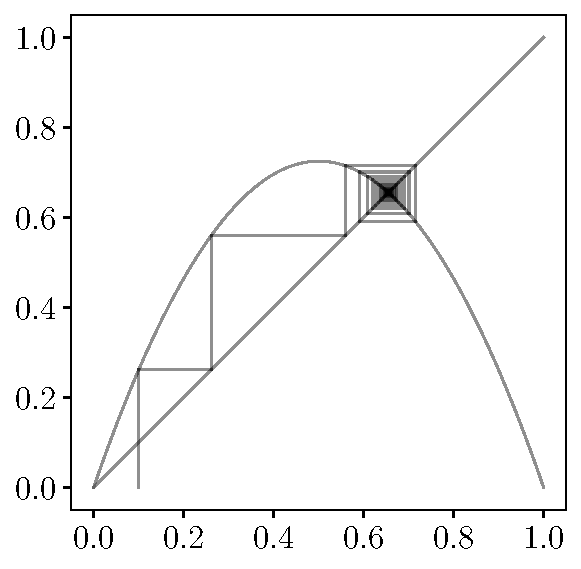
\includegraphics[width=6cm]{cobweb_0.1_2.9.pdf}
    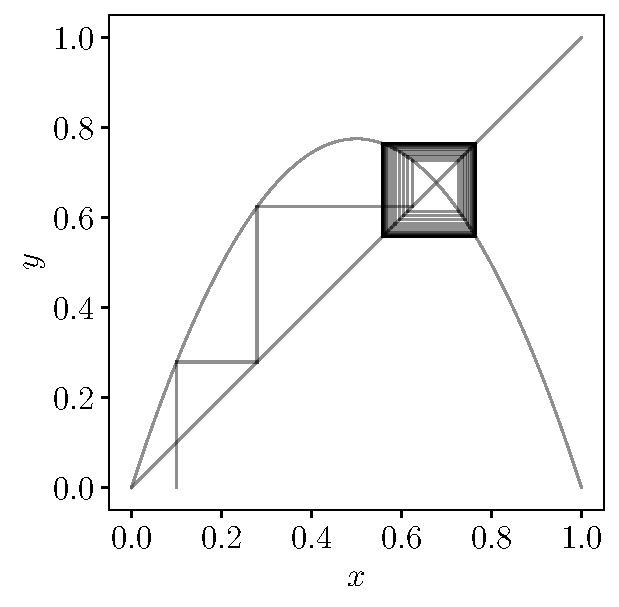
\includegraphics[width=6cm]{cobweb_0.1_3.1.pdf}
    \caption{So called cobweb plots of the logitic family $F\mu(x) = \mu x(1-x)$ for $\mu = 2.9$ and $\mu = 3.1$ respectively. Displays the long term behaviour of the orbit of $x_0 = 0.1$ over successive iterations of $F_\mu$. When $\mu = 2.9$ an attracting fixed point is clearly visible and when $\mu = 3.1 > \mu_1$ an attracting period 2 point can be seen.}
    \label{fig:cobweb_2.9_3.1}
\end{figure}

Here the attracting fixed point at $x = x_\mu$ decays into a repellor and a period-2 attractor emerges around the point $\mu_1 = 3$. This can been seen clearly in Figure \ref{fig:cobweb_2.9_3.1} which shows the long term stability of the orbit. This behaviour we have just outlined is called a \emph{bifurcation}, specifically a \emph{period-doubling bifurcation} and the point $\mu_1 = 3$ is called a \emph{bifurcation point}. The next bifurcation point happens at $\mu_2 = 1 + \sqrt{6}$ whereby the stable period-2 attractor decays into a repellor and a period-4 attractor emerges. It turns out that there are many bifurcations as $\mu$ increases towards value of four. The value of $\mu$ at which the $k$-th bifurcation occurs is denoted $\mu_k$. The bifurcations occur ever closer together in what is called a \emph{period-doubling cascade}, until the whole system becomes in some sense chaotic. Figure \ref{fig:bifurcation_2.8} shows what is called a bifurcation diagram, which plots the stable orbits of $x$ as $r$ increases. From the bifurcation diagram we can clearly see the initial bifurcation at $\mu_1 = 3$ whereby the initial attracting fixed point $x = x_\mu$ decays into a repellor and the period-2 attractor $x = x_{\mu_2}$ emerges. Again the second bifurcation at $\mu_2 = 1 + \sqrt{6}$ is shown whereby the period-2 attractor $x = x_{\mu_2}$ decays into a repellor and a period-4 attractor emerges. These bifurcations cascade as $\mu$ increases until at a certain point called the \emph{accumulation point} ($\mu_\infty = \mu \approx 3.56995$) whereby periodicity transforms suddenly into chaos as slight pertubations in the starting value $x$ cascade into large changes over a iterations of $F_\mu$. A chaotic orbit for when $\mu > \mu_\infty$ can be seen in Figure \ref{fig:cobweb_3.5_3.9}. An interesting property of the period-doubling cascade is the ratio between bifurcation interval to the next bifurcation interval between each period doubling calculated using \[\delta_k  = \frac{\mu_k - \mu_{k-1}}{\mu_{k+1}-\mu_k}\]It turns out that as $k \to \infty$ this ratio converges to a constant $\delta \approx 4.66921$ called the \emph{Feigenbaum constant}. A remarkable discovery is that this constant holds for the bifurcations of every one-dimensional map with a only one quadratic maximum. Looking back at the logistic map a rather strange result from the bifurcation diagram is the presense of small isolated intervals of stability present amongst the chaos. These intervals are referred to as \emph{islands of stability}. The point $\mu = 1 + 2\sqrt{2}$ is the start of one such interval in which a period-3 attractor emerges from the chaos. However, once again a period-doubling cascade happens and the system decends back into chaos. For $\mu > 4$ no attractors exist and the whole system becomes unstable.
\begin{figure}[h]
    \centering
    \includegraphics[width=14cm]{bifurcation_2.8.png}
    \caption{Bifurcation diagram of the logitic family $F\mu(x) = \mu x(1-x)$ for $2.8 \leq r \leq 4.0$.}
    \label{fig:bifurcation_2.8}
\end{figure}

\begin{figure}[h]
    \centering
    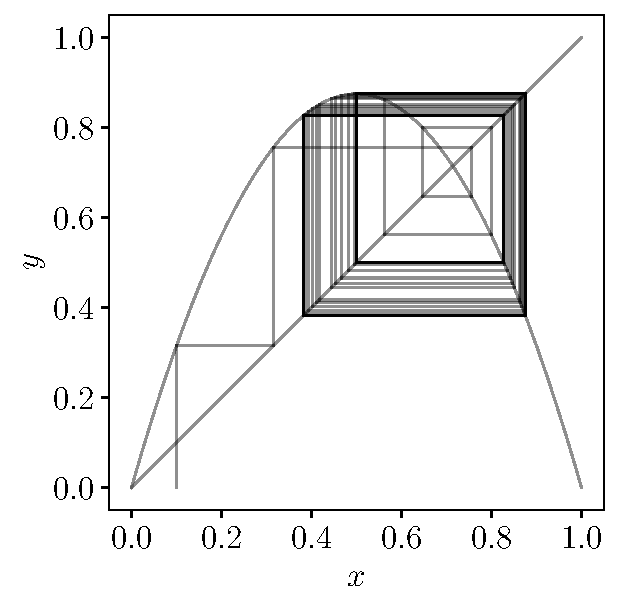
\includegraphics[width=6cm]{cobweb_0.1_3.5.pdf}
    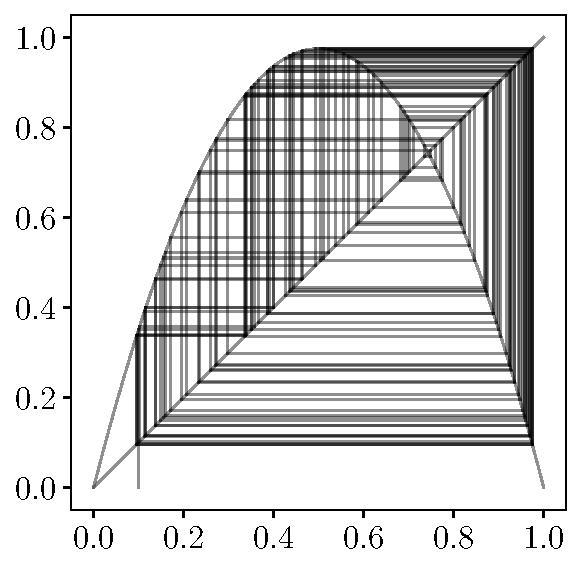
\includegraphics[width=6cm]{cobweb_0.1_3.9.pdf}
    \caption{Cobweb plots of the logitic family $F\mu(x) = \mu x(1-x)$ for $\mu = 3.5$ and $\mu = 3.9$ when $x_0 = 0.1$ respectively. When $\mu = 3.5 > \mu_2$ an attracting period-4 point is visible. For $\mu = 3.9 > \mu_\infty$ $F_\mu$ has infinite periodicity and has become visibly chaotic.}
    \label{fig:cobweb_3.5_3.9}
\end{figure}

\section{Sharkovsky's Theorem and Type}
Sharkovsky's theorem \cite{sharkovsky} is an hugely important theorem to chaotic dynamical systems. It states that in continous maps on the real numbers periodic points of all periods can occur and that the presense of a periodic point of given period implies the existence of other periods by a total ordering called \emph{Sharkovsky's Order}. First we will introduce a theorem that proves the existence of fixed points on closed intervals of the real numbers. This theorem is a simplified version of \emph{Brouwer's fixed-point theorem} \cite{brouwer}. The full theorem is used to prove the existence of fixed points when a continuous map is applied to compact, convex sets.
\begin{thm} \label{thm:fixed-points}
    Let $I$ be a closed interval on $\mathbb{R}$ and suppose $f: I \to I$ is continuous. Then $f$ has a fixed point.
    \begin{proof}
        Let $g(x) = f(x) - x$ and $I = [a, b]$ for $a, b \in \mathbb{R}$. Since $f(x)$ is continuous, $g(x)$ is continuous. As $f$ is a map $f(a) \in I$, hence $g(a) \geq 0$. Similarly, $f(b) \in I$, so $g(a) \leq 0$. By the Intermediate Value Theorem there exists some $x \in I$ with $a \leq x \leq b$ such that $g(x) = 0$. Hence $f(x) = x$.
    \end{proof}
\end{thm}

A similar fixed-point theorem that we shall use in a later is as follows. This proof however states the existence of a fixed point in a specific interval $I \subseteq \mathbb{R}$.

\begin{thm} \label{thm:interval-fixed-points}
    Let $I$ be a closed interval on $\mathbb{R}$ and suppose $f: \mathbb{R} \to \mathbb{R}$ is continous with $I \subseteq f(I)$. Then $f$ has a fixed point in $I$.
    \begin{proof}
        Let $I = [a, b]$ where $a, b \in \mathbb{R}$. Since $I \subseteq f(I)$ there exits $c, d \in I$ such that $f(c) = a$ and $f(d) = b$. Suppose $g(x) = f(x) - x$, then $g(x)$ is continuous. Also $g(c) = a - c \geq 0$ and $g(d) = b - d \leq 0$. By the Intermediate Value Theorem there exists some $x \in I$ with $a \leq x \leq b$ such that $g(x) = 0$. Hence $f(x) = x$.
    \end{proof}
\end{thm}

First we will prove a special case of Sharkovsky's theorem. This theorem was discovered by Li and Yorke in their paper \emph{'Period Three Implies Chaos'} \cite{li-yorke}. Now we can start to prove this special case of Sharkovsky's theorem by Li and Yorke. The proof below is adapted from work by Devaney, Chapter 1.10 \cite{devaney}.

\begin{thm}\label{thm:period3chaos}
    Let $I$ be a closed interval on $\mathbb{R}$ and suppose $f: I \to I$ is continuous. If $f$ has a point of period three then $f$ has periodic points of all other periods.
    \begin{proof}
        Before we begin the proof lets make some simple observations:
        \begin{enumerate}[(i)]
            \item If $I, J$ are closed intervals with $I \subseteq J$ and $J \subseteq f(I)$ then by Theorem \ref{thm:interval-fixed-points} $f$ has a fixed point in $I$.
            \item If $A_0, A_1, \cdots$ are closed intervals with $A_{i+1} \subseteq f(A_i)$ for $0 \leq i \leq n - 1$ then there exists a subinterval $J_0 \subseteq A_0$ such that $f(J_0) \subseteq A_1$. Similarly, there exists a subinterval $J_1 \subseteq A_1$ such that $f(J_1) \subseteq A_2$. Hence there exists a subinterval $J_1 \subseteq J_0$ such that $f(J_1) \subseteq A_1$ and $f^2(J_1) = A_2$. Continuing we get a nested sequence of intervals which are mapped in order into each $A_i$. Hence there exists some $x \in A_0$ such that $f^i(x) \in A_i$ for all $i$.
        \end{enumerate}
        To begin the proof let $a, b, c \in \mathbb{R}$ with $f(a) = b$, $f(b) = c$ and $f(c) = a$. Assume wlog that $a < b < c$. Let $I_0 = [a,b]$ and $I_1 = [b,c]$. Hence $I_1 \subseteq f(I_0)$ and $I_0 \cup I_1 \subseteq f(I_1)$. By Theorem \ref{thm:fixed-points} $f$ has a fixed point between $b$ and $c$. Similarly, $f^2$ has at least one fixed point between $a$ and $b$. Hence $f$ has a point of period 2. Now let $n \geq 2$. Define the nested sequence of intervals $A_0, A_1, \cdots, A_{n-2} \subseteq I_1$ inductively. Let $A_0 = I_1$. Since $I_1 \subseteq f(I_1)$, there exists a subinterval $A_1 \subseteq A_0$ and $f(A_1) = A_0 = I_1$. Furthermore there exists a subinterval $A_2 \subseteq A_1$ such that $f(A_2) = A_1$ and therefore $f^2(A_2) = A_0 = I_1$. Continuing we get a subinterval $A_{n-2} \subseteq A_{n-3}$ such that $f(A_{n-2}) = A_{n-3}$. By our second observation $x \in A_{n-2}$ then $f(x), f^2(x), \cdots, f^{n-2}(x) \subseteq A_0$ so $f^{n-2}(A_{n-2}) = A_0 = I_1$. As $I_0 \subseteq f(I_1)$ there exits a subinterval $A_{n-1} \subseteq A_{n-2}$ such that $f^{n-1}(A_{n-1}) = I_0$. Since $I_1 \subseteq f(I_0)$, $I_1 \subseteq f^n(A_{n-1})$ so that $f^n(A_{n-1})$ covers $A_{n-1}$. Hence by our first observation $f^n$ has a fixed point $p$ in $A_{n-1}$. The first $n-2$ iterates of $p$ are in $I_1$, the $n-1$th iterate is in $I_0$ and the $n$th is $p$. If $f^{n-1}(p)$ is in the interior of $I_0$ then $p$ has period $n$. However, if $f^{n-1}(p)$ is in the boundary of $I_0$ then $n = 2$ or $3$.
    \end{proof}
\end{thm}

This consequences of this theorem are remarkable. If you can find a point of period three for a map $f$ then there exists periodic points of all other periods, hence periodic points exist with infinite periods. Further note that the only assumption we have made for $f$ is that it is continous and speaks to the generality of this result. This theorem however does not show the bigger picture of whats going on here, for this we need to introduce Sharkovsky's theorem, but first we need explain Sharkovsky's order.

\begin{defn}
    The total ordering on $\mathbb{N}$ defined below is named \emph{Sharkovsky's order}. \[ 3 \rhd 5 \rhd 7 \rhd 9 \rhd \cdots \rhd 2 \cdot 3 \rhd 2 \cdot 5 \rhd \cdots \rhd 2^2 \cdot 3 \rhd 2^2 \cdot 5 \rhd \cdots \rhd \cdots \rhd 2^3 \rhd 2^2 \rhd 2 \rhd 1 \]
\end{defn}
(i.e. first all the odd integers multiplied by $2^k$ for $k \in \mathbb{N}$. This exhausts all the natural numbers apart from powers of two, which are then ordered last in descending order.) This brings us to Sharkovsky's theorem.

\begin{thm}
    Let $I$ be a closed interval on $\mathbb{R}$ and suppose $f: I \to I$ is continuous. If $f$ has a periodic point of period $k$ then for all integers $l \rhd k$, $f$ has periodic points of period $l$.
\end{thm}

The proof of this theorem will be ommited since it is outwith the scope of this paper, however can be found here \cite{sharkovsky}. Hence from above and noticing the Sharkovsky ordering it can be seen that if $f$ has a periodic point whose period is not a power of two, then $f$ has infinitely many many periodic points. The converse statement also holds. If $f$ has finitely many periodic points then they all must have periods that are powers of two. This sort of behaviour was present in the logistic family with the period doubling bifurcations in Section \ref{sec:logistic_maps}. Furthermore the logistic maps perodicity follows the Sharkovsky's ordering in reverse. Furthermore when all periods are present and we have reached the end of Sharkovsky's ordering the system becomes chaotic. It can be seen that this theorem is a generalised of Theorem \ref{thm:period3chaos} discovered by Li and Yorke \cite{li-yorke} as period three is the greatest period in Sharkovsky's ordering hence its presense implies the existence of all other periods. It can be useful to catagorise maps defined on a closed interval based on their periods. This leads us to the next definition which is based on work by Ruette, Section 3.3 \cite{ruette}.

\begin{defn} \label{def:type}
    Let $I$ be a closed interval on $\mathbb{R}$ and suppose $f: I \to I$ is continuous. Let $n \in \mathbb{N} \cup \left\lbrace 2^{\infty} \right\rbrace$. An interval map is of \emph{type} $n$ if the periods of periodic points of $f$ are the set $\left\lbrace m \in \mathbb{N} : m \unrhd n \right\rbrace$, where $\left\lbrace m \in \mathbb{N} : m \unrhd 2^\infty \right\rbrace$ means $\left\lbrace 2^k : k > 0 \right\rbrace$.
\end{defn}

\begin{exmp} \label{exmp:piecewise_sharkovsky}
    Let $f: [0, 4] \to [0, 4]$ be a piecewise linear map with $f(0) = 2$, $f(2) = 3$, $f(3) = 1$, $f(1) = 4$ and $f(4) = 0$. This graph of $f$ is shown in Figure \ref{fig:piecewise_linear}. Clearly $f$ is continuous. It can be seen that the point 0 is a period-$5$ point. Moreover $f^3[0, 1] = [1, 4]$, $f^3[1, 2] = [2, 4]$ and $f^3[3, 4] = [0, 3]$. So $f^3$ has no fixed points in those intervals. However $f^3[2, 3] = [0, 4]$ hence by by Theorem \ref{thm:interval-fixed-points} $f^3$ has at least one fixed point in $[2, 3]$. Moreover $f: [2, 3] \to [1, 3]$, $f: [1, 3] \to [2, 5]$ and $f: [1, 4] \to [0, 4]$ are all monotonically decreasing on $[2, 3]$. Therefore $f^3$ is monotonically decreasing on $[2, 3]$ and so the fixed point is unique. Therefore this can only be the fixed point for $f$, and as such no period 3 point exists. Hence by Sharkovsky's theorem the map $f$ contains periodic points with the period of every natural number apart from 3. Therefore using Definition \ref{def:type} it is clear that $f$ is of type $5$.

    \begin{figure}[h]
        \centering
        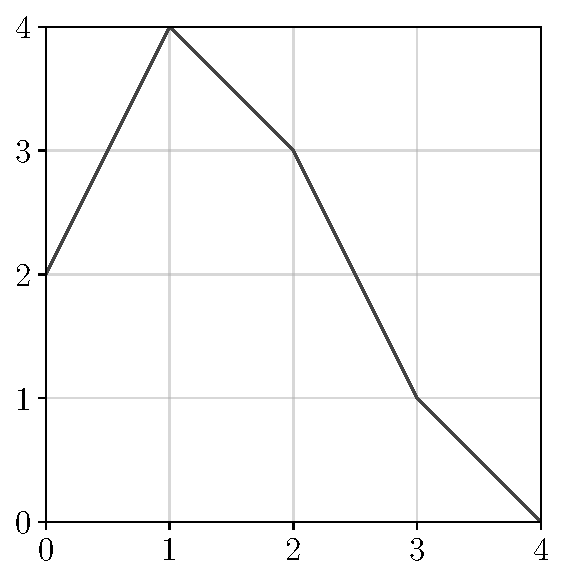
\includegraphics[width=5cm]{piecewise_0_4}
        \caption{Piecewise linear map $f$ with a period five point.}
        \label{fig:piecewise_linear}
    \end{figure}

\end{exmp}

Sharkovsky subsequently proved that continous maps defined on intervals of the reals can constructed to be of any type \cite{sharkovsky} \cite{sharkovsky2}. In his proof he constructs orbits for odd periods, even periods then periods that conside of powers of two separately. However the construction to prove that continous interval maps of any odd type can be created is similar to a more general version of Example \ref{exmp:piecewise_sharkovsky}. This theorem is termed Sharkovsky's Realisation Theorem and is stated below. This theorem uses an elegant proof discovered by Alseda, Llibre, and Misiurewicz \cite{alm} and outlined by Burns and Hasselblatt here \cite{burns-hasselblatt} using a family of continous maps called the trunctated tent maps.

\begin{thm}
    Every tail of the Sharkovsky order is the set of periods for some continuous map of an interval into itself.
    \begin{proof}
        Let $T_h: [0, 1] \to [0, 1]$ where $T_h(x) = min(h, 1-2|x-1/2|)$ be the family of truncated tent maps with $0 \leq h < 1$.
    \end{proof}
\end{thm}

\section{Topological Conjugacy}


\section{Defining Chaos}
The term \emph{chaos} in Mathematics is vauge and has multiple definitions. The main definition we will be working with comes from Devaney \cite{devaney} and takes a strictly topological approach. Before we introduce this key definition however we first need to set up some preliminary definition. This first definition helps build an understanding of the dense, complex nature of chaos.
\begin{defn}
    A map $f: I \to I$ is \emph{topologically transitive} if for every pair of non-empty open sets $U, V \subseteq I$ there exists $k > 0$ such that $f^k(U) \cap V \neq \emptyset$.
\end{defn}
Stated another way, in a topologically transitive map, points in an arbitraily small neighbourhood can be mapped to any other arbitrary neighbourhood under repeated a number of applications of the mapping. 

\begin{prop} \label{prop:dense-transitive}
    Let $f: I \to I$ be a map with $x \in I$. If $\mathcal{O}(x)$ is dense then $f$ is topologically transitive.
    \begin{proof}
        Let $U, V \subseteq I$ with $U, V \neq \emptyset$. Let $x \in I$ such that $\overline{\mathcal{O}(x)} = I$. Then there exists $k, l \in \mathbb{N}$ such that $f^k(x) \in U$ and $f^l(x) \in V$. Assume $k > l$, then $f^k(x) \in f^{k - l}\left( \mathcal{O}_{f^l}(x) \right)$ and therefore $f^k(x) \in U \cap f^{k-l}(V)$. Hence $f$ is transitive.
    \end{proof}
\end{prop}

It can also be seen that in specific cases, such as compact subsets of $\mathbb{R}$ or $S^1$ the converse statement is also true. This next definition emphasises the erratic, uncontrollable and unstable nature of chaos.

\begin{defn}
    A map $f: I \to I$ has \emph{sensitive dependence on initial conditions} if there exists a $\delta > 0$ such that, for all $x \in I$ and any neighbourhood $N$ of $x$, there exists $y \in N$ and $k \geq 0$ such that $\left\lvert f^k(x) - f^k(y) \right\rvert > \delta$.
\end{defn}

In other words there exist points arbitrary close to $x$ that eventually get mapped at least $\delta$ far apart under multiple applications of the map. Hence this definition states that small pertubations in the mappings input may eventually increase to become wildly different over time. However this definition is not enough on its own to characterise chaos. Here is an example of a non-chaotic discrete system with sensitive dependence on initial conditions.

\begin{exmp} \label{exmp:2x}
    Let $f: \mathbb{R} \to \mathbb{R}$ with $f(x) = 2x$. Let $\delta < 2^k \varepsilon$ and suppose $|x - y| = \varepsilon$, then $\left\lvert f^k(x) - f^k(y) \right\rvert = \left\lvert 2^k x - 2^k y \right\rvert = 2^k \left\lvert x - y \right\rvert = 2^k \varepsilon > \delta$. Hence we can always choose $k$ large enough so that this holds and so $f(x) = 2x$ has sensitive dependence on initial conditions.
\end{exmp}

This next example fufills our first definition of being topologically transitive, however is not sensitive to initial conditions. To understand this next example however, we will need to introduce the following theorem.

\begin{thm} \label{thm:s1irrational}
    Let $\lambda \in \mathbb{R}$ and $T_\lambda(\theta) = \theta + 2\pi \lambda$. Each orbit of $T_\lambda$ is dense in $S^1$ if $\lambda$ is irrational.
    \begin{proof}
        Let $\theta \in S^1$ and suppose $\lambda$ is irrational. If $T_\lambda^n(\theta) = T_\lambda^m(\theta)$ then $(n - m)\theta \in \mathbb{Z}$ and so $n = m$. Since $S^1$ is compact every infinite subset of points on $S^1$ must have a limit. Hence if $\varepsilon > 0$ then there exists $n, m \in \mathbb{Z}$ such that $\left\lvert T_\lambda^n(\theta) - T_\lambda^m(\theta) \right\rvert < \varepsilon$. Let $k = m - n$, then $\left\lvert T_\lambda^k(\theta) - \theta \right\rvert < \varepsilon$. By definition $T_\lambda$ preserves distance in $S^1$ and since $T_\lambda^k$ maps the arc connecting $\theta$ and $T_\lambda^k(\theta)$ to the arc connecting $T_\lambda^k(\theta)$ and $T_\lambda^k(2 \theta)$ with length also less than $\varepsilon$. Therefore $\left\lbrace \theta, T_\lambda^k(\theta), T_\lambda^k(2 \theta), \cdots \right\rbrace$ partition $S^1$ into arcs of length less than $\varepsilon$ Hence this orbit is dense.
    \end{proof}
\end{thm}

Now using this theorem we can prove the following example.
\begin{exmp}
    The rotations $T: S^1 \to S^1$, $T_\lambda(\theta) = \theta + 2\pi \lambda$ where $\lambda$ is irrational are topologically transitive by Theorem \ref{thm:s1irrational} and Proposition \ref{prop:dense-transitive}. However, since the mappings are distance preserving, they are not sensitive to initial conditions.
\end{exmp}


The map in Example \ref{exmp:2x} is clearly a map we would never consider to be chaotic as the dynamics of this system are easily explained. Hence our definition of chaos must include more than just a sensitive dependence on initial conditions. Using these definitions we have established we can finally give an exact definition of chaos in a discrete dynamical system.

\begin{defn}
    A map $f: I \to I$ is \emph{chaotic} on the set $I$ if all of the following hold:
    \begin{itemize}
        \item[(i)]$f$ has sensitive dependence on initial conditions.
        \item[(ii)]$f$ is topologically transitive.
        \item[(iii)]periodic points of $f$ are dense in $I$.
    \end{itemize}
\end{defn}

\chapter{Higher-Dimensional Dynamical Systems}
\section{Stability in Higher Dimensions}

\chapter{Defining Chaos}
\section{Chaos in Higher Dimensions}
\chapter{Chaotic Attractors}

\chapter{Fractals}
\section{Julia Sets}

\bibliography{chaos}

\end{document}